\documentclass[12pt,oneside,a4paper]{article}

\usepackage{./custom}

\usepackage[backend=biber]{biblatex}
\addbibresource{./biblio.bib}

\begin{document}

\begin{titlepage}
\begin{center}


\includegraphics[scale=0.5]{./img/logo_centralesup.jpg} \hfill

\includegraphics[scale=0.3]{./img/logo_digiplante.png}

\vfill 

\textsc{\Large Projet enjeu : Santé et biotechnologies}\\[0.5cm]

\vfill

\textsc{\Large \'Etude documentaire et bibliographique}\\[1.5cm] 

% Title
\HRule \\[0.4cm]
{ \LARGE \bfseries Développement d'outils mathématiques \\ 
   pour l'agriculture de précision \\[0.4cm] }

\HRule \\[1.5cm]

\vfill

{\large
\begin{center}
  \textbf{Client et RP} \\~\\
\begin{tabular}{rl}
   \quad Pierre &\textsc{Carmier} \\
    \quad Paul-Henry &\textsc{Courn\`ede} \\
  
\end{tabular}
\end{center}
\vfill
\begin{center}
  \textbf{Groupe SBT-11(P2018)} \\~\\
  
\begin{tabular}{rl}

    \quad John &\textsc{de Wasseige} \\
    \quad Nayef &\textsc{Derwiche} \\
    \quad Alexis &\textsc{Mathey} \\
    \quad Daina &\textsc{Zheng} \\ \\
\end{tabular}
\end{center}
}

\vfill

{\large \today}

\end{center}
\end{titlepage}
\newpage

\tableofcontents
\newpage

\section{Résumé}

On résumera ici les enjeux, l'objectif et le livrable du projet défini avec le client
et les principales conclusions de l'étude bibliographique.
\newpage
\section{\'Etude bibliographique}

Afin d'avoir une première approche globale du sujet, 
nous commençons par introduire
le concept d'agriculture de précision et son rôle de plus en plus important.
Il semble en effet important de commencer par expliquer \emph{pourquoi}
des laboratoires comme Digiplante existent et plus généralement \emph{pourquoi}
faire des progrès dans le domaine de l'agriculture de précision est nécessaire.

On présente ensuite des concepts généraux sur la physiologie des plantes
ainsi que la réaction de photosynthèse, critique dans la création
de biomasse.
Ceux-ci permettront par la suite de comprendre plus aisément
les modèles mathématiques utilisés pour décrire la croissance des plantes.

Une fois le contexte général posé, nous expliquons l'histoire de la modélisation 
des plantes. Ceci va nous permettre de comprendre quelles ont été les différentes 
sources d'influences tout au long de l'étude de la modélisation des plantes.

On décrira finalement le modèle LNAS appliqué au blé, ceci en se rappelant que l'objectif poursuivi est de prédire le rendement
de la biomasse totale de la plante.


\subsection{Concepts d'agriculture de précision}
La croissance exponentielle de la population~\cite{wiki:popu_mondiale}
au cours des dernières décennies et par conséquent le besoin de nourrir
tout le monde, ne laisse pas d'autres choix
si ce n'est celui d'optimiser l'agriculture.
Cependant le concept d'optimisation de l'agriculture peut 
paraître assez flou et général.
Une définition assez intuitive d'une agriculture optimisée
peut être d'essayer d'obtenir
les récoltes les plus bénéfiques en ayant une consommation minimum d'énergie
et d'intrants (eau, engrais\dots) en tenant compte de facteurs à la fois
agronomiques, environnementaux et économiques~\cite{wiki:agri_prec}.

C'est précisemment ce que vise l'agriculture de précision.
Globalement, on dira que \enquote{l'agriculture de précision désigne
l'ensemble des techniques culturales basées sur l'utilisation
des nouvelles technologies de mesure et de traitement de l'information
spatialisée}~\cite{jullien2005agriculture}.

À ce jour les coûts engendrés par les installations technologiques
nécessaires pour utiliser les systèmes d'agriculture de précision
mais l'investissement est souvent rentabilisé à long, surtout 
dans le cas de grandes parcelles.
En effet, cette nouvelle forme d'agriculture ne permet pas seulement
d'être bénéfique pour les sols et nappes phréatiques,
elle engendre également une diminution des dépenses de l'agriculteur
par une consommation moins importante d'engrais et d'eau.
À cet diminution d'utilisation d'engrais s'associe une réduction
d'émissions de particules néfastes pour
environnement telles que des nitrates, phosphates
et pesticides~\cite{emission_agri_particules}.
Ce dernier point semble d'autant plus important dans le contexte
écologique actuel où le respect de l'environnement est nécessaire
d'un point vue légal mais aussi moral.

\begin{figure}
  \begin{center}
    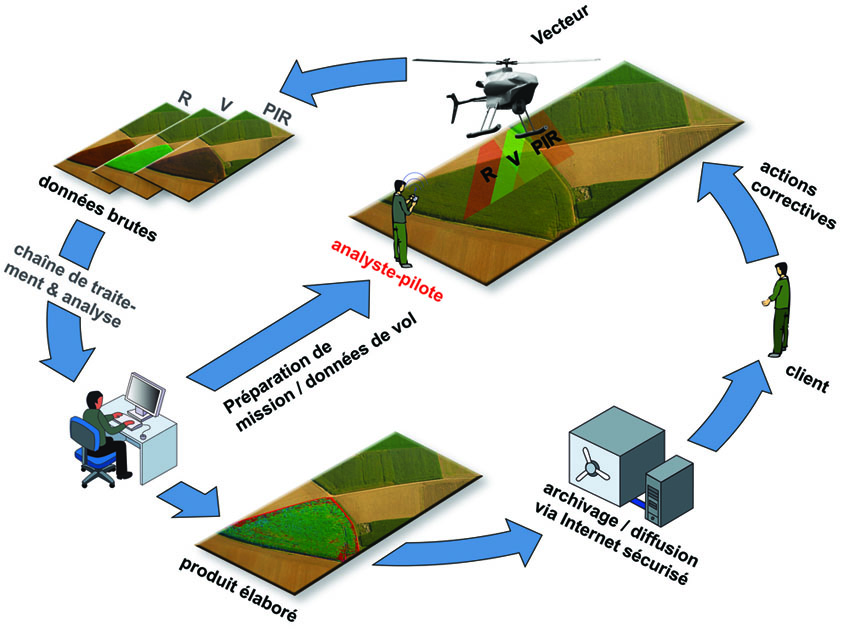
\includegraphics[scale=0.42]{./img/agridrone.jpeg}
  \end{center}
  \caption{Représentation d'une application d'agriculture de 
  précision~\cite{vegedrones}.
  On retrouve un système d'acquisition d'images sur drones ainsi
  qu'une analyse rétroactive des données récupérées.}
\end{figure}
\subsection{Historique de la modélisation de la croissance des plantes}
+++++ INTRODUCTION SUR LES 4 SOUSSOUSSECTIONS ++++ \\
Cette section reprend la démarche suivie dans 
l'article \emph{Une histoire de la modélisation des plantes}, \textsc{Cournède} et al., 2009~\cite{histoire_mod_plantes}.

\subsubsection{Débuts de la botanique et de l'agronomie}
L’étude des plantes a très tôt été un domaine privilégié du savoir humain.
Les plantes en effet sont un élément majeur des écosystèmes dans lesquels l’homme évolue. Elles sont source de nourriture, de remèdes, de médicaments,
de matériaux, d’esthétique. 
Enfin, elles sont un objet scientifique d’intérêt qui a très tôt aiguisé le sens de l’observation, l’esprit d’analyse, de synthèse, de déduction des hommes. 
La connaissance des plantes s’est accrue lors de l’histoire des hommes, qui ont développé la cueillette, l’agriculture, l’usage des plantes
médicinales. 
La connaissance et l’inventaire des variétés de plante ont ainsi été des
enjeux majeurs car ils permettaient la connaissance de nouveaux remèdes
et étaient sources de nourritures et matériaux. 
L’homme a aussi cherché à regrouper, croiser, faire croître 
et conserver les espèces qui lui sont utiles.

La botanique, issue de l’étude de l’anatomie des plantes,
est une science très ancienne.
En témoignent les traités de classification de plantes, comme ceux
d’Aristote (vers -300), ou encore l’inventaire et la description de
centaines de plantes médicinales par Dioscoride (1er siècle),
ainsi que les traités chinois qui inventorient les espèces utiles à
l’agriculture et à la médecine traditionnelle avec de premiers efforts
de classification. 
Efforts de classification qui se poursuivront vraiment en Europe à partir du
XVIIème siècle avec les premières distinctions par famille, par genre,
par espèce, par structure de graine (\emph{Les éléments de Botanique} par
Joseph Pitton de Tournefort en $1656-1708$, \emph{Systema naturae} en 1735
et \emph{Philosophia botanica} en 1751 par Linné et les travaux de la
famille de Jussieu pendant le XVIIIème siècle).
Ces classifications ne sont pas objectives, 
elles sont le fruit d’un raisonnement \emph{empirique}.

En parallèle, l’agronomie se développe au XVIIème siècle en Europe
et s’intéresse au processus de croissance et développement des plantes.
Des travaux d’abord très pratiques sont réalisés sur des méthodes agricoles 
(labour, ensemencement, taille, greffes…), notamment ceux de
Jean-Baptiste de la Quintinie et d'Olivier de Serres.

Au XIXème, les processus biologiques commencent à être étudiés de façon plus
précise, en particulier la provenance du carbone, de l’azote,
de l’oxygène et de l’eau dans la plante.
On s'intéresse également aux problématiques de nutrition et
au rôle de organes, comme en témoignent les ouvrages
\emph{Recherces chimiques sur la végétation} de Théodore de Saussure en 1804.
Quelques années plus tard, on découvre la respiration, la photosynthèse
et sa fameuse équation
\begin{equation}
	\ce{6CO2 + 6H2O + \text{énergie solaire} -> C6H12O6 + O2 }.
  \label{eq:photosynthese}
\end{equation}

La physiologie, science qui étudie le fonctionnement des plantes,
se sépare alors de la botanique qui se contente de les classifier.

\subsubsection{Les premiers modèles}

La modélisation mathématique précise (qui va au-delà de la simple
description qualitative et fournit une description quantitative
avec des capacités prédictives) n’arrive pas tout de suite en biologie. 
Le développement de la biologie n’a pas suivi le même schéma que celui de
nombreuses autres sciences comme la physique, où l’observation a permis de
tirer des concepts quantitatifs au niveau macroscopique
(loi de Mariotte par exemple) avant de les expliquer par des lois qui s’appliquent au niveau microscopique (Boltzmann). De même pour la mécanique, l’optique, l’électricité avec des applications qui n’ont pas eu à attendre la compréhension au niveau atomique. La biologie végétale par contre a paradoxalement été mieux comprise au niveau cellulaire et microscopique sans que des lois précises macroscopiques en soient tirées.

Trois types de modèles vont se développer et vont changer cela : les modèles de l’architecture botanique, les modèles de production en agronomie et les modèles géométriques en informatique. Ainsi la convergence de ces trois modèles initialement séparés va permettre récemment les débuts de la modélisation précise de la croissance des plantes à la fin du XXème siècle.  

L’architecture botanique va considérer la structure des plantes non plus comme une description statique issue de la classification traditionnelle mais comme le résultat de l’organogénèse des méristèmes, la cinétique de mise en place des axes feuillés, en se basant sur une combinatoire des modes de croissance, de ramification et de floraison. (Francis Hallé et Roelof Oldeman).

En parallèle, l’agronomie s’est attaquée à la prédiction de la production surfacique de biomasse. Les modèles hollandais comme celui de De Witt (1970) en sont les précureurs. On ne considère plus la plante en elle-même mais la surface foliaire au mètre carré LAI \footnote{LAI : Leaf Area Index, ratio entre la surface totale supérieure des feuilles vertes et la surface de sol sur laquelle se développe la culture} et la production végétale par mètre carré. Les organes ne sont plus considérés individuellement mais par compartiments. A chaque compartiment est allouée une certaine quantité de la biomasse créée en fonction de sa force de 
puits\footnote{La force de puits d'un organe est proportionelle à la quantité de biomasse qui sera allouée à cet organe.\cite[~p.229--231]{hopkins2003physiologie} 
Ainsi, on écrit intuitivement 
\[
	\text{force de puits} = \text{taille du puits} * \text{activité du puits}
\]
}. 
Les agronomes ont ainsi montré que la production de biomasse est proportionnelle au LAI, ainsi qu'à l’énergie utile de la lumière incidente : PAR \footnote{PAR : photosynthetically active radiation }, à la lumière interceptée : I et à un facteur d’efficience énergétique : LUE\footnote{LUE : Light Use Efficiency}. On se reporte à la loi de Beer-Lambert pour trouver la quantité de lumière interceptée, qu'on note I : 

\[ I = 1-e^{-k\cdot\mathrm{LAI}} \]

Ce qui permet ensuite de trouver la production de biomasse $Q$
en déterminant le LUE et en mesurant la PAR.
\[ 
  Q = \mathrm{LUE}\times\mathrm{PAR}\times I 
\]

Dernier concept empirique développé, celui de temps thermique. En effet, si on modélise la croissance de la plante  en fonction du temps, cette croissance est très irrégulière et se fait par à coup. Mais si l’on considère le temps thermique\footnote{Le temps thermique correspond à l'accumulation de températures dépassant un certain seuil :
\[
\tau^{(n+1)} = tau^{(n)} + max[0, \underline{T^{(n)}} - T_c], 
\]
où \underline{T^{(n)}} est l'écart de température constaté et 
T_c est le seuil de variation de température qu'on impose.
} 
on peut trouver une relation quasi-linéaire.

\subsubsection{Informatique et modèles géométriques}

L’arrivée des ordinateurs a révolutionné les méthodes de simulation et de modélisation des systèmes et l’étude des plantes en a bien sûr profité.
Les ordinateurs ont fait leur apparition en même temps presque que les modèles agronomes et botaniques. Ainsi très vite ils ont été vus comme un moyen de simuler la structure géométrique complexe des plantes avec le développement d’arbres combinatoires, binaire et fractals. Mais ces structures purement géométriques et trop rigides ne simulent pas encore bien le développement complexe des plantes.
Les travaux d’Aristide Lindenmayer aboutissent à une grammaire au formalisme puissant, grammaire générative basée sur le principe de réécriture \cite{LSystem}.

L’arrivée des ordinateurs a révolutionné les méthodes de simulation et de modélisation des systèmes et l’étude des plantes en a bien sûr profité.
Les ordinateurs ont fait leur apparition en même temps presque que les modèles agronomes et botaniques. Ainsi très vite ils ont été vus comme un moyen de simuler la structure géométrique complexe des plantes avec le développement d’arbres combinatoires, binaire et fractals. Mais ces structures purement géométriques et trop rigides ne simulent pas encore bien le développement complexe des plantes.
Les travaux d’Aristide Lindenmayer aboutissent à une grammaire au formalisme puissant, grammaire générative basée sur le principe de réécriture.

\noindent{
\fbox{
  \parbox{\textwidth}{\paragraph{Qu'est-ce qu'un L-Système?}
Un L-Système est noté :
\[ \{ V,S,\omega ,P \}  \]
Une grammaire formelle qui comprend :
\begin{itemize}
\item Un ensemble alphabet \textbf{V}: Ensemble de variable du L-Système
\item Un ensemble de constantes \textbf{S} : Ensemble de constantes servant notamment lors du dessin géométrique.
\item Un axiome de départ $\mathbf{\omega}$ : État initial.
\item Un ensemble de règles \textbf{P} : Règles de production.
\end{itemize}
Un exemple simple : Algues de Lindenmayer
\[ 
  \left\lbrace
		\begin{array}{cl}
		  V &= \{ A, B\} \\
		  S &= \{ \} \\
		  \omega &= A \\
		  P &= ( A\rightarrow AB)\wedge (B\rightarrow A) \\	
     \end{array}
   \right. 
\]
Avec le résultat sur 6 générations :

\begin{itemize}
  \item[$\bullet$] $n=0$, A
  \item[$\bullet$] $n=1$, AB
  \item[$\bullet$] $n=2$, AB A
  \item[$\bullet$] $n=3$, AB A AB
  \item[$\bullet$] $n=4$, AB A AB AB A
  \item[$\bullet$] $n=5$, AB A AB AB A AB A AB
  \item[$\bullet$] $n=6$, AB A AB AB A AB A AB AB A AB AB A
\end{itemize}

Une suite de symbole générée par L-Système peut être prise en entré par un programme informatique qui s’en servira pour générer une structure géométrique, le plus simple étant d’utiliser un turtle en 2D voire en 3D, ou encore dans un langage orienté objet avec des pointeurs on peut générer une chaine cellulaire qui évolue. Les symboles dans V sont les parties des plantes dessinées et les symboles dans S donnent des informations sur la façon dont elles sont dessinées, leur orientation par exemple.
}   
}

Ces modèles de L-système conviennent bien à la simulation des structures des plantes, elles marchent d’autant mieux combinées à la notion de temps thermique qui ordonne la dynamique de croissance et permettent d’aboutir in fine à une architecture fidèle. Mais elles n’intègrent pas la notion de production de biomasse et si elles permettent de prédire une structure finale aussi fidèle que possible, elles ne permettent pas de prédire le rythme de production. Les écophysiologistes se sont alors efforcés d’intégrer des mécanismes de plus en plus fins, avec une simulation locale et géométrique de la photosynthèse, des échanges entre organes par un système de transport-résistance avec la notion de force de puits de organes puits qui puisent la biomasse produite par les organes sources etc… Ces systèmes complexes qui permettent enfin une simulation fine au niveau individuel ne sont pourtant pas adapté à la simulation et encore moins la modélisation d’un grand ensemble de plantes et ceux pour deux raisons : 
\begin{enumerate}
\item \emph{Le coût en ressources de calcul :} il croît avec le temps de la simulation et le nombre d’individus considérés, encore plus si l’on doit considérer les interactions entre les individus.
\item \emph{La difficulté à paramétrer :} dû au grand nombre de paramètre notamment par rapport aux données que l’on peut raisonnablement récolter.
\end{enumerate}

\subsubsection[Le modèle GreenLab]{Le modèle GreenLab : entre modèle individuel et modèle de production}

\begin{figure}[h]
	\begin{center}
	
	
  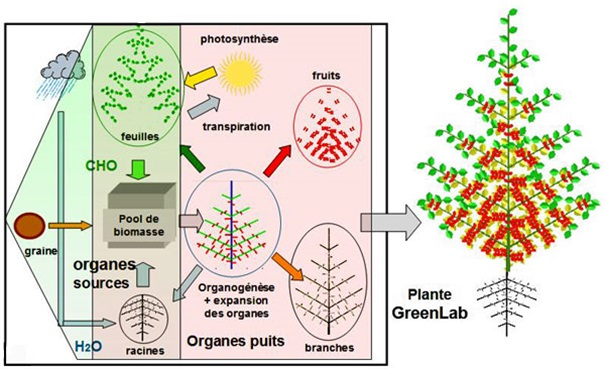
\includegraphics[scale=1.0]{./img/sGL.jpg}
  \caption{Schéma Type d'un modèle GreenLab}
  \label{fig:schémaGL}
  
  \end{center}
\end{figure}


Le modèle GreenLab propose une alternative. Il reprend des simplifications utiles du modèle agronome au niveau de la production : La prise en compte de l’architecture individuelle de la plante n’est pas utile au niveau d’un champ, mais la connaissance de la distribution des différents organes à différents moment est vitale. Autrement dit, les aspects géométriques peuvent être négligés mais pas la composition quantitative des structures. On fait alors l’hypothèse d’un pool de biomasse commun dans lequel les organes vont piocher, et on ne considère que la photosynthèse net, ie les proportions de glucides qui sert effectivement à la construction de matière sèche des organes. 

Au niveau de l’allocation cette approche décrit précisément des compartiments d’organes se comportant de façon similaire, ce qui rend l’allocation de biomasse plus facile à modéliser entre organes sources et organes puits et permet de se passer d’une description géométrique ou même topologique (graph) exhaustive. Les organes sont générés par cohortes (groupes générés en même temps) de même type grâce à des équations de production des méristèmes selon leur âge physiologique, et des lois de probabilités qui déterminent la croissance, la sénescence et le branching. Et comme tous les organes d’une même cohorte d’organe du même type ont le même état, on peut opérer facilement une factorisation en sous-structures qui rend les calculs plus léger, ainsi le temps de calcul n’est plus proportionnel au nombre d’organe mais seulement à l’âge de la plante. En particulier en multipliant le nombre d’organe de chaque cohorte par la force de puit correspondante et additionnant le tout on obtient la demande de la plante.

Ensuite l’augmentation $\delta q$ de biomasse de chaque organe est obtenu avec la formule suivante :

\[ \delta q = \phi \cdot Q/D \]

Avec $\phi$ la force de puit, Q la pool de biomasse global et D la demande totale de la plante.

La masse des organes est la somme cumulée de l’augmentation des biomasse, on peut obtenir rapidement les dimensions (longueur, diamètre, surface) des organes en utilisant de simples lois géométriques (beaucoup plus simple que celles utilisées lorsque la géométrie est prise en compte dans la production). 

Puis pour que le cycle se répète, la biomasse des compartiments s’obtient  en sommant les cohortes de même organes, en particulier on peut obtenir la masse du feuillage puis la surface foliaire ce qui permettra de déterminer la production de biomasse au prochain cycle. La boucle est bouclée.

Pour résumer, Ce modèle est un modèle dynamique de croisance des plantes qui marche par rétroaction entre croissance (production de biomasse) et développement (allocation quantitative et architecture). Le calcul de la production ne prend que peu en compte l’architecture de la plante mais seulement l’équation global de production et les relations sources-puits ce qui permet des économies de calcul intéressante et n’empêche pas dans un second temps de générer des structures géométriques fidèles issus d’un modèle de production simplifié mais robuste. Ainsi la plasticité des plantes est très bien représenté par ce modèle et on peut rendre compte de différent phénotypes d’une même espèce dans deux environnement très différents.

\begin{figure}[h]
	\begin{center}
	
	
  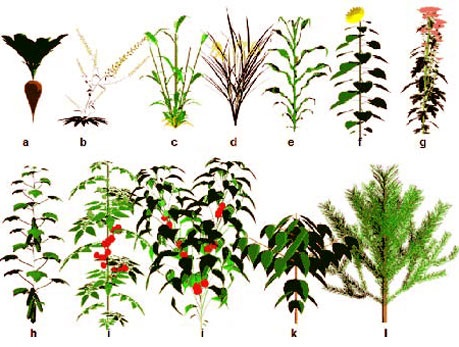
\includegraphics[scale=1.0]{./img/exempleGL1.jpg}
  \caption{Exemple de plantes générées grâce à GreenLab}
  \label{fig:exempleGL1}
  
  \end{center}
\end{figure}

Cela permet notamment la visualisation en image de synthèse très fidèles et complexes de plantes dont la croissance a été modélisé sans prendre en compte le détail géométrique de cette même structure, donc avec un temps de calcul très intéressant. L’augmentation de biomasse de chaque organe a déjà été simplement déterminée grâce aux équations précédentes, dont on déduit également la forme et le volume, de simples règles géométriques positionnent ces organes dans l’architecture selon l’empilement des entre-nœuds autour d’un axe, la phyllotaxie, l’angle de branchement, la courbure des axes… \ref{fig:exempleGL1}

On peut même simuler des paysages entiers grâce à ces méthodes, avec le raffinement des paysages fonctionnels qui prennent en compte finement les interactions plantes-environnement, la distribution des ressources hydriques et des radiations lumineuses entre plantes qui sont en compétition etc… \ref{fig:exempleP1} \ref{fig:exempleP2}

\begin{figure}[h]
	\begin{center}
	
	
  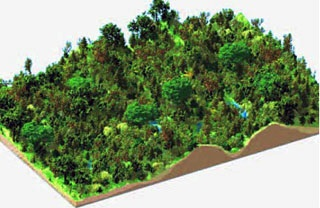
\includegraphics[scale=1.0]{./img/exempleP1.jpg}
  \caption{Paysage fonctionnel avec environnement aux paramètres (radiations, humidité) simulés}
  \label{fig:exempleP1}
  
  \end{center}
\end{figure}

\begin{figure}[h]
	\begin{center}
	
	
  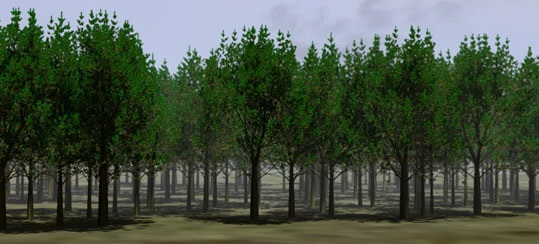
\includegraphics[scale=1.0]{./img/exempleP2.jpg}
  \caption{Paysage fonctionnel généré grâce à GreenLab}
  \label{fig:exempleP2}
  
  \end{center}
\end{figure}




\subsection{Fonctionnement et développement de la plante}

\subsubsection{Généralités}

Tout d'abord, présentons succintement comment se développe et fonctionne une plante. 
C'est la morphogénèse qui décrit l'ensemble des mécanismes qui participent à l'édification d'un organsime vivant.

Chez les plantes, la morphogénèse commence avec la germination de la graine et s'arrète à la mort de la plante.~\cite[p.~22]{these_modelisation}.
Celle-ci diffère d'une plante à l'autre, et dépend également de l'environnement de la plante.

Ce sont les méristèmes\footnote{Le méristème est un tissu formé de cellules indiffériencées (embryonnaires) qui se divisent activement et permettent la croissance.} qui permettent à la plante de se développer, en allongeant des organes déjà existants ou en créant de nouveaux organes.
Lors de la germination de la graine, au stade embryonnaire, des méristèmes permettent déjà le développement de la plante (méristèmes racinaires, caulinaires).
On distingue les méristèmes végétatifs, à l’origine des organes végétatifs (tige, feuilles, racines) et les méristèmes reproducteurs, à l’origine des fleurs.
On distingue également les méristèmes primaires, qui permettent à la plante de croître en longueur (tiges et racines) et les méristèmes secondaires, qui permettent la croissance en épaisseur de la plante.
La création de nouveaux organes est réalisée par alignement de nouvelles briques élémentaires (formée par les méristèmes), constituées :
\begin{itemize}
	\item d'un noeud, auquel sont liés les feuilles
	\item d'un entrenoeud 
	\item d'un bourgeon situé à la base du noeud, à l'aisselle des feuilles
\end{itemize} 

Ces briques élémentaires sont appelées phytomères. Cette caractéristique permet de simplifier la modélisation de la croissance d'une plante.



\subsubsection{Photosynthèse}


Sans doute que la particularité la plus intéressante des plantes, et qui justifie le mieux leur étude est leur capacité à synthétiser de la matière organique (des glucides...) à partir de \ce{CO2}, d'eau et d'énergie solaire. C'est la célèbre photosynthèse qui permet ainsi à la plante de \textit{transformer de la matière minérale en matière organique}, qu'on peut présenter selon cette équation : 
\[
	\ce{6CO2 + 6H2O + \text{énergie solaire} -> C6H12O6 + O2 }
\]
Tous les éléments de la plante participent à ce processus de photosynthèse :
\begin{itemize}
	\item les racines puisent dans le sol l'eau et les sels minéraux nécessaires		
	\item les feuilles captent l'énergie solaire et le dioxyde de carbone 
  (grâce aux cellules chlorophiliennes 
  et aux stomates\footnote{Orifice de petite taille situé sur les feuilles 
  qui permet les échanges gazeux entre l'air et la plante.})
\end{itemize}

\begin{figure}[h]
	\begin{center}
  
\includegraphics[scale=0.51]{./img/photosynthese.jpg}
  \caption{Photosynthèse}
  \label{fig:photosynthèse}
	\end{center}
\end{figure}

Les sucres ainsi formés apportent l'énergie nécessaire au fonctionnement de la plante et assurent son développement en permettant la synthèse de cellulose qui est l'élément consitutif principal des plantes.
On identifie ainsi les éléments qui agissent sur la croissance de la plante : 
\begin{itemize}
	\item la lumière
	\item l'eau
	\item le dioxyde de carbone
	\item la température : car la température agit sur l'ouverture des stomates et donc sur le flux des échanges gazeux
	\item l'azote, qui permet à la plante de construire les acides aminés nécessaires à l'élaboration des protéines
	\item d'autres minéraux, comme le potassium qui favorise les transferts au sein de la plante
\end{itemize}

Tous les organes de la plante s'unissent donc pour aboutir à la production de biomasse. Cette biomasse est ensuite distribuée aux organes pour permettre leur développement.

Parce que ce mécanisme permet de synthétiser de la matière minérale en matière organique et de capter du \ce{CO2}, gaz à effet de serre notoire, il est crucial de comprendre ce mécanisme de photosynthèse. C'est pourquoi il est, au même titre que la croissance des plantes l'objet de nombreuses recherches (avec comme application : créer de l'électricité propre en dissociant \ce{H2O} en Oxygène et en Hydrogène, capter du \ce{CO2}...




\newpage
\section{modèle LNAS}
Ci-dessous est un exemple de blé en appliquant le modèle LNAS.
\[ {Q_o^{(n+1)}} = (1-\beta_o^{(n)}-\gamma_o^{(n)} )(Q_o)^{(n)} +\alpha_o^{(n)}q^{(n)} \]
Pour des feuilles jaunes, comme ils étaient les sénilités des feuilles verts donc ils ne reçoivent pas de biomasses qui viennent de Q, la production de biomasse. Dans ce cas, 
\[ {Q_y^{(n+1)}}=(1-\gamma_y^{(n)})Q_y^{(n)}+Y_l^{(n)}Q_l^{(n)} \]
Le temps thermique du jour n+1 peut s'écrire:
\[ {\tau}^{(n+1)}=\tau^{(n)}+max[0,T_-^{(n)}-T_c] \]
Supposant que la répartiotion de biomasse ne commence qu'après passer le temps caractéristique $\tau_g$ et  nous pouvons paramétrer la fonction $\alpha$ avec la loi log-normal:
\[ {\alpha_g^{(n)}}=F_{\log N(\mu_s,\sigma_g)}(\tau^{(n)}-\tau_g)=\frac{1}{2} (1+erf[\frac{1}{\sigma_g \sqrt{2}}\log (\frac{\tau^{(n)}-\tau_g}{t_{1/2}-\tau_g})]) \]
De même pour la fonction $\beta $ et $\gamma$, on a
\[ {\beta_o}=\eta_o F_{\log N(\mu_l, \sigma_l)}(\tau-\tau_l) \]
\[ {\gamma_l}=(1-\eta_l)F_{\log N(\mu_l, \sigma_l)}(\tau-\tau_l) \]
\[ {\gamma_y}=F_{\log N(\mu_y, \sigma_y)}(\tau-\tau_y) \]

\[ {q^{(n)}}=RUE min[SSI^{(n)}, TSI_\uparrow^{(n)}]PAR^{(n)}(1-e^{-\lambda LAI^{(n)}})+\sum_o \beta_o^{(n)}Q_o^{(n)} \]
\begin{itemize}
\item $\mathrm{Q}(n)$ : Production de biomasse au jour n par unité de surface.
\item $\o=$ $\left\lbrace grain, stem,root,greenleaf\right\rbrace$ :différent partie de blé
\item $\alpha$  :fonction de répartition
\item $\beta_o$  :fonction de reutilisation
\item $\gamma$ : fonction de sénilité
\item $q^{(n)}$: production de biomasse par photosynthèse au jour n 
\item $\mu_g=\log (\tau_{1/2}-\tau_g)$
\item $\sigma_g$: variance de lq distribution
\item $\tau_{1/2}$ : temps thermique où $\alpha_g$ vaut 1/2
\item $erf(x)$: fonction d'erreur
\item $\eta_o$: fraction de biomasse 
\item $RUE$ :efficience de conversion
\item $\mathrm{PAR}(t)$ : quantité de radiations photosynthétiquement actives par unité de surface
\item $LAI^{(n)}$ : facteur d'apres loi de Beer-Lambert 
\item $SSI^{(n)}$: index de pression stomatique 
\item $TSI^{(n)}$: index de pression thermique
\end{itemize}
L'équation d'équilibre de l'eau
\[ {R^{(n+1)}}=R^{(n)}+W^{(n)}-Es^{(n)}-Tp{(n)}-d{(n)}\]
L'eau dans la terre dépend du profondeur z,
\[ {R^{(n)}}=\int_0^{z_M}dz \theta^{(n)}(z) \]
L'évaporation et transpiration sont exprimées comme
\[ {Espot^{(n)}}=K_sET0^{(n)}e^{-\lambda LAI^{(n)}}\]
\[ {Tppot^{(n)}}=K_cET0^{(n)}(1-e^{-\lambda LAI^{(n)}})\]
\begin{itemize}
\item $R^{(n)}$: l'eau dans la terre du jour n
\item $W^{(n)}$ : l'eau d'irrigations et  précipitations au jour n
\item $Es^{(n)}$: l'eau perdu par évaporation vanant de la terre
\item $Tp$: transpiration
\item $d$: fonction qui compte le fait la saturation d'eau dans la terre
\end{itemize}

\newpage
\subsection{Développement et évaluation des modèles de croissance des plantes et implémentation sur la plateforme Pygmalion.}

\subsubsection{Généralités}

Les modèles mathématiques de modélisation de la croissance des plantes sont généralement caractérisés par un grand nombre de processus en interaction,  un grand nombre de paramètres et une acquisition coûteuse des données expérimentales. 
Nous présentons ici succintement Cette complexité rend la modélisation très difficile. Le but de cette thèse est de présenter et proposer de bonnes pratiques de modélisation, de donner un aperçu global des différentes étapes de modélisation dans le cadre de la croissance des plantes.
Le modèle LNAS (celui sur lequel on travaillera en premier dans le cadre du projet enjeu) est présenté comme illustration de ces méthodes, ici appliqué à la betterave, et montre comment il peut être paramétré, évalué et appliqué à la prédiction des rendements, et ce à travers des données expérimentales réelles. Ce modèle a d’intéressante capacité de prédiction lorsqu’il est couplé a de bonnes méthodes d’acquisition de données.

\subsubsection{Caractéristiques propres aux modèles de croissance de plantes}

\begin{itemize}

\item \textbf{Une complexité importante} au niveau des processus et des paramètres
\item \textbf{Une paramétrisation difficile} à cause de cette complexité ainsi que du coût important des données.
\item \textbf{Un besoin croissant} en techniques sophistiquées en informatiques, mathématiques et statistiques.
\item \textbf{Une importante diversité} de modèles existants sans benchmarking entre les différentes approches (lacune de méta-études statistiques)

\end{itemize}

Les solutions mathématiques et statistiques classiques et généralistes ne sont pas immédiatement adaptées à la modélisation des plantes et nécessitent un travail d’adaptation important pour prendre en compte ses spécificités.

D’un autre côté les logiciels de modélisations spécialisés, bien que performant, ne prennent pas assez en compte l’aspect paramétrisation et évaluation statistiques.

Les logiciels développés récemment dans ce domaine offrent des solutions intéressantes mais elles sont peu compatibles entre elles et limitent donc la comparaison, le benchmarking des modèles.

L’objectif est donc à la fois bien de situer les bonnes pratiques de modélisation, et de proposer une implémentation pratique, notamment à travers la plateforme Pygmalion en C++ qui fournit un template générique de modèle, des structures de données, des méthodes, des classes et framework appropriés, ainsi qu’une méthodologie statistique.

\subsubsection{Bonnes pratiques en modélisation}

\begin{itemize}

\item \textbf{Analyse du modèle :} Etude des comportements généraux du modèle, au niveau théorique et numérique par des simulations. Pour déterminer les données nécessaires à la paramétrisation, et faire une analyse de sensibilité pour repérer les paramètres importants.
\item \textbf{Identification du modèle :} Confronter les modèles à des données expérimentales. Identification de la structure : pour identifier dans la famille du modèle la plus intéressante. Identification des paramètres : pour identifier la valeur des paramètres pour la structure choisie.
\item \textbf{Evaluation du modèle :} Vérifier qualitativement (comportement générale et aptitude de simulation) et quantitativement (comparaison aux données réelles) si le modèle atteint ses objectifs, c’est-à-dire vérifier la correspondance aux donnée actuelles (goodness of fit), tester ses capacités prédictives et évaluer son niveau d’incertitude.

\end{itemize}

\textbf{Ces étapes ne sont pas linéaires :} des allers retours sont nécessaires pour ajuster finement le modèle.

Ensuite ces étapes sont appliquées au modèles LNAS avec des jeux de données expérimentales, avec succès, en notant des capacités prédictives intéressantes dans un cadre données expérimentales très différent de celui utilisé lors de la calibration du modèle.

Cette première étape développée par le laboratoire MAS de l’ECP, montre l’intérêt de la démarche, et invite à l’appliquer avec d’autres modèles, d’autres plantes et sur d’autre jeux de données tout en continuant d’améliorer la plateforme, tout en simplifiant son utilisation.

\newpage
\subsection{Analyse de sensibilité}
L'analyse de sensibilité d'un modèle permet d'évaluer la sensibilité de la
variable réponse à des perturbations dans les entrées du modèle et
d'identifier les paramètres ayant le plus d'influence
sur les résultats du modèle.

En supposant que le modèle qui peut se représenter suivant:
\[
  y = f(z_1,\dots,z_p)
\]
avec $z_1,\dots ,z_p$ les paramètres dont on veut étudier l'influence sur $y$.

Généralement on distingue deux types de méthodes quantitatives:
\begin{description}
  \item[les\ méthodes\ locales] Elles permettent d'étudier l'effet de la
variation locale d'un facteur $z_i$ avec tous les autres facteurs étant fixés à des valeurs moyennes qui en général sont peu coûteuses en temps de calcul
\item[les\ méthodes\ globales], où on autorise tous les paramètres à varier simultanément dans leur intervalle de variation. Ces méthodes permettent d'identifier et d'évaluer des interaction entre les paramètres
\end{description}
 décomposition de la variance V du modèle en termes de dimension croissance pour analyse la sensibilité:
\[ {V}=\sum_{i=1}^pV_i+\sum_{1\leq i,j \leq p} V_{ij}+\cdots +V_{1\cdots p}\]

\[ {V_i}=Var(E(y|Z_i))\]

\[ {V_{ij}}=Var(E(y|Z_i,Z_j))-V_i-V_j \]

\[ {V_{1\cdots p}}=V-\sum_{i=1}^p V_i-\sum_{1\leq i,j \leq p}-\cdots -\sum_{1\\leq i_1<\dot <i_{p-1}\leq p} V_{i_1 \cdots i_{p-1}} \]
On défit ensuite les indices de sensibilité correspondants:
\begin{itemize}
\item $S_i=\frac{V_i}{V}$: l'indice du premier ordre qui permet d'évaluer chaque facteur individuellement
\item $S_ij=\frac{V_ij}{V}$: l'indice du premier ordre qui permet d'évaluer quantitativement l'effet d'interaction entre deux facteurs
\end{itemize}
En appliquant cette méthode aux systèmes dynamiques dont les sorties sont multidimensionnelles, impliquant le calcul d'indice de sensibilité $S_i^j(t)$ à chaque jour t pour chaque composante $y_j$ de la variable $y$.
Donc l'indice de sensibilité généralisé du paramèter i  pour la composante $y_j$ :
\[ {s_i^j}=\frac{\sum_{t=1}^TS_i^j(t)Var(y_j(t))}{\sum_{t=1}^T Var(y_j(t))} \]
\newpage
\section{Contexte du projet}
\newpage
\section{Organisation du groupe}
Nous présenterons dans cette section l'organisation générale du groupe.
On abordera d'abord les outils que nous avons utilisés pour partager notre travail
le plus efficacement possible.
On présentera ensuite notre gestion de la bibliographie.
On détaillera finalement l'organisation interne du groupe,
plus précisemment le système mis en place pour optimiser la communication
ainsi que la manière dont les tâches ont été réparties pendant ce premier semestre.

\subsection{Outils de travail collaboratif}
Pour des raisons pratiques et esthétiques, nous avons décider d'écrire
nos rapports en \LaTeX.
Il s'agissait donc de trouver la meilleure façon de partager le code source
et de pouvoir contrôler les changements apportés au document.
Une première idée pourrait être d'utiliser ShareLaTeX qui propose une plate-forme
de compilation en ligne ainsi qu'un système de gestion de versions
assez simple à utiliser.
Nous n'avons pas choisi cette solution notamment pour les raisons suivantes.
L'utilisateur doit être connecté dès qu'il veut travailler sur le projet,
le système de compilation est assez lent et l'utilisateur n'est pas libre
d'utiliser son éditeur de texte ou son visualisateur de \textsc{pdf} favori.

Pour palier aux problèmes décrits ci-dessus, le logiciel \texttt{git}
associé à GitHub est une très bonne alternative.
Il permet en effet à chaque membre du groupe de travailler sans être connecté
ainsi que d'utiliser son éditeur et compilateur favori.
Chaque membre travaille donc de son côté en faisant des \emph{commits}
et lorsqu'il juge que son travail est utile pour les autres, 
il \emph{push} sur le serveur.
L'algorithme du fusion, \emph{merge}, permet également de fusionner intelligemment
les lignes d'un fichier qui ont été modifiées par plusieurs membres.
Le dernier point à souligner est que \texttt{git} permet une gestion des branches,
particulièrement pratique lorsqu'on veut développer une partie du projet
sans risquer de créer des erreurs dans le programme principal.

Nous l'utilisons pour implémenter un programme en \textsc{Julia}
pour le client dont le code source est sur la plate-forme GitLab.
Nous avons également un dossier sur
GitHub\footnote{\url{https://github.com/jdewasseige/projet-sbt11}}
qui contient nos fichiers pour rédiger l'étude documentaire.

\subsection{Gestion de la bibliographie}
Pour la gestion de la bibliographie au sein du document,
nous utilisons le package \texttt{biblatex}.
Celui-ci permet d'écrire l'ensemble de nos références dans un document \texttt{.bib}
sous la forme suivante.
\begin{verbatim}
  @online{histoire_mod_plantes,
    title = {Une histoire de la modélisation des plantes},
    author = {Philippe de Reffye and Marc Jaeger 
    and Paul-Henry Cournède},
    url = {https://interstices.info/jcms/c_38032/une-histoire-de-
    la-modelisation-des-plantes},
    year = {2009},
    month = "04",
  }
\end{verbatim}
La mise en page est alors automatique en fonction des informations fournies
et le rendu de l'exemple est présenté ci dessous.
\begin{figure}[h]
  
\includegraphics[scale=0.6]{./img/rendu_elem_bib.jpg}
\end{figure}

Cela parait à priori assez lourd d'écrire soi-même toutes les informations
en suivant cette syntaxe mais il existe des logiciels comme Zotero
qui font le travail à notre place.
Les sources trouvées sur Google Scholar peuvent également être exportées
aisément au format \texttt{BibTex}.
           
\subsection{Organisation et partage des tâches}
Il nous reste un dernier point à décrire, celui de la \emph{communication}
au sein du groupe.
Nous utilisons Slack\footnote{\url{https://slack.com/}} qui est un logiciel
de plus en plus utilisé pour les travaux de groupe ainsi que dans les start-ups.
Il permet d'éviter de devoir alterner entre plusieurs applications comme les mails,
DropBox et Twitter, puisqu'il permet d'être connecté
à celles-ci au sein de l'application.
On peut également créer plusieurs \emph{channels} pour séparer la communication
entre les différentes tâches.
Par exemple dans ce projet nous avons les \emph{channels} suivantes :
\texttt{general}, \texttt{etude-documentaire}, 
\texttt{planning} et \texttt{dev\_plate-forme}.
On trouve aussi un système d'historique et de gestion de fichiers efficace.

Le partage de tâches est associé au planning qui se trouve
dans l'Annexe~\ref{ann:planning} à la page~\pageref{ann:planning}.

\subsection{Risques, difficultés et problèmes potentiels}
Nous avons identifié plusieurs risques, difficultés et problèmes qui pourrait survenir durant le projet et ralentir sa mise en oeuvre: 

\begin{itemize}
	\item Une perte partielle ou totale de nos données, à cause d'une mauvaise manipulation sur les plateformes de travail, dont le contenu peut être modifié/supprimé par chaque utilisateur.
	\item Nous n'arrivons pas à acquérir les compétences informatiques nécessaires pour implémenter et travailler sur les modèles informatiques de modélisation de plantes.
	\item Un seul élève du groupe réalise la plupart du travail (parce qu'il est le seul à savoir coder par exemple). Cela conduirait à une perte de communication et de motivation au sein du groupe.
	\item Peu de communication avec notre client, et en conséquence mauvaise compréhension du projet et de ses objectifs. 
\end{itemize}

Pour éviter que cela n'arrive, nous allons :
\begin{itemize}
	\item utiliser la plateforme GitHub qui permet de récupérer les sauvegardes précédentes.
	\item nous partager équitablement les tâches
	\item faire en sorte que chaque membre du groupe comprenne chacune des étapes de notre travail.
	\item échanger et essayer de rencontrer régulièrement notre client, profitant de sa proximité, étant chercheur au laboratoire MAS de Centrale.
\end{itemize}
\newpage
\section*{Conclusion}
\addcontentsline{toc}{section}{Conclusion}

Les perspectives qu'offre l'étude de la croissance des plantes sont des plus stimulantes.
En effet, les enjeux sont cruciaux. Les plantes sont un élément clé de notre économie. A la base de nos régimes alimentaires, elles sont également source d'oxygène, d'énergie avec l'émergence des agro-carburants, et sont utilisées dans la construction, l'industrie des vêtements et même dans l'industrie pharmaceutique.

Dans le même temps, pour répondre à une demande de plus en plus forte, l'agriculture a recours à l'irrigation intensive, aux engrais et aux pesticides pour augmenter ses rendements. Malheureusement, ces méthodes ont un impact négatif sur l'environnement et leur utilisation n'est pas viable, comme en témoigne par exemple le quasi-asséchement de la mer d'Aral à cause d'une culture intenisive du coton~\cite{aral}
 
Heureusement, la science, aidées des mathématiques et d'une collecte de données devenue omniprésente, semble plus que jamais capable de développer une agriculture viable et productive. Pour cela, elle bénéficie de plusieurs siècles d'études des plantes qui ont permis d'affiner leurs connaissances.



\newpage
\section{Remerciements}
\newpage

%\documentclass{ctexart}
\usepackage{tikz}
\usetikzlibrary{trees}
\tikzset{box/.style={rectangle ,rounded corners=5pt, draw}}
\begin{document}
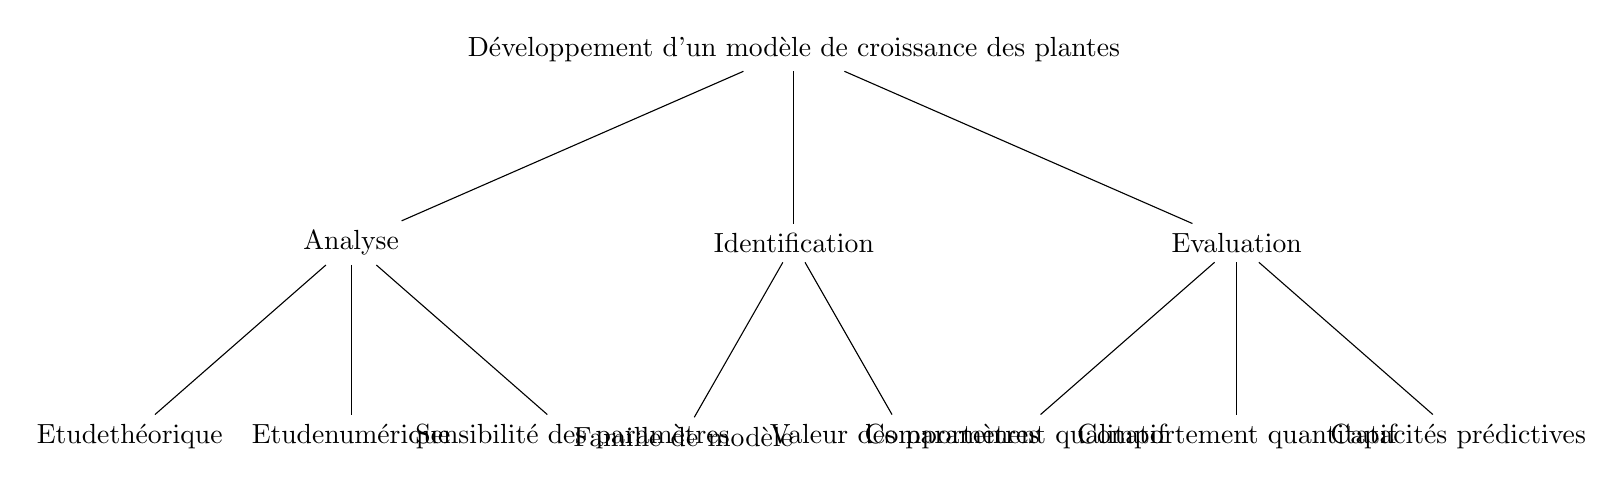
\begin{tikzpicture}[level distance=70pt, sibling distance=5pt]
  
\tikzstyle{level 1}=[sibling distance=160pt]
\tikzstyle{level 2}=[sibling distance=80pt]
\tikzstyle{level 3}=[sibling distance=200pt]
%\tikzstyle{level 4}=[sibling distance=50pt]
%\tikzstyle{level 5}=[sibling distance=80pt]
%\tikzstyle{level 6}=[sibling distance=50pt]
%\tikzstyle{level 7}=[sibling distance=80pt]
%\tikzstyle{level 8}=[sibling distance=50pt]
%\tikzstyle{level 9}=[sibling distance=80pt]

\node{Développement d’un modèle de croissance des plantes}
  child { node {Analyse}
    child { node {{Etude\\ théorique}} }
    child { node {Etude \\ numérique}}
    child { node {Sensibilité des paramètres}}
    }
    child { node {Identification}
    child { node {{Famille de modèle}} }
    child { node {Valeur des paramètres}}
    }
    child { node {Evaluation}
    child { node {{Comportement qualitatif} }}
    child { node {Comportement quantitatif}}
    child { node {Capacités prédictives}}
    };
\end{tikzpicture} 
\end{document}
%\newpage

\addcontentsline{toc}{section}{Bibliographie}
\nocite{*}
\printbibliography
\newpage

\appendix
\part*{Annexes}
\section{Planning}
\label{ann:planning}

\end{document}